\chapter{Plan of Work}

\subsection{Development and Report Milestones}

Illustrated on the next page is a gantt chart reflecting our goals relative
to the project deadlines. It incorporates both core development and report items.
For our initial stages we focus on environment and platform set-up (i.e.
deploying a development webserver) and the initial, core code implementation. At
the same time we will finalize the details of our final product via the report
milestones. \\ 

{\bfseries Development milestones} have been spread out following the completion 
of the first eport on 22 February 2013, beginning with deploying our development
 environment and server through Heroku from which we continue to our next 
 milestone of deploying Ruby on Rails as well as all the Gems and API packages we are incorporating into our project, most notably Yahoo! Finance. \\

{\bfseries Report milestones} are also set concurrently. As we begin to initialize
our development environment, we will also build on top of and expand on previous
reports to expand upon and fully realize the details of {\textit Capital Games}. \\

%{\bfseries Core goals leading up to Demo 1} include establishing all core 
%functionality for {\textit Capital Games}. This includes the following:
%\begin{itemize}
%\item {\bfseries Rails framework-deployed core functionality :} This
%includes a working system for navigating the website, registering a new
%user account, logging in, and creating as well as participating in leagues.
%\item {\bfseries Setting a foundation for the database: } On top of having 
%the aforementioned core functionalities, they also must be able to pass
%data through a routed database.  
%\item {\bfseries Implementing the Yahoo! Finance API: }
%\item {\bfseries A functional user interface:} Our website should be useable, 
%and having a functional user interface from the start will give us a lot of
%room to expand and optimize the UI. \\
%\end{itemize}


\subsection{Dario's Stuff Here re: distribution of labor}

Coming soon to a tex file near you!



\hfil\eject \pdfpagewidth=8.5in \pdfpageheight=16in
\begin{figure}
\centering
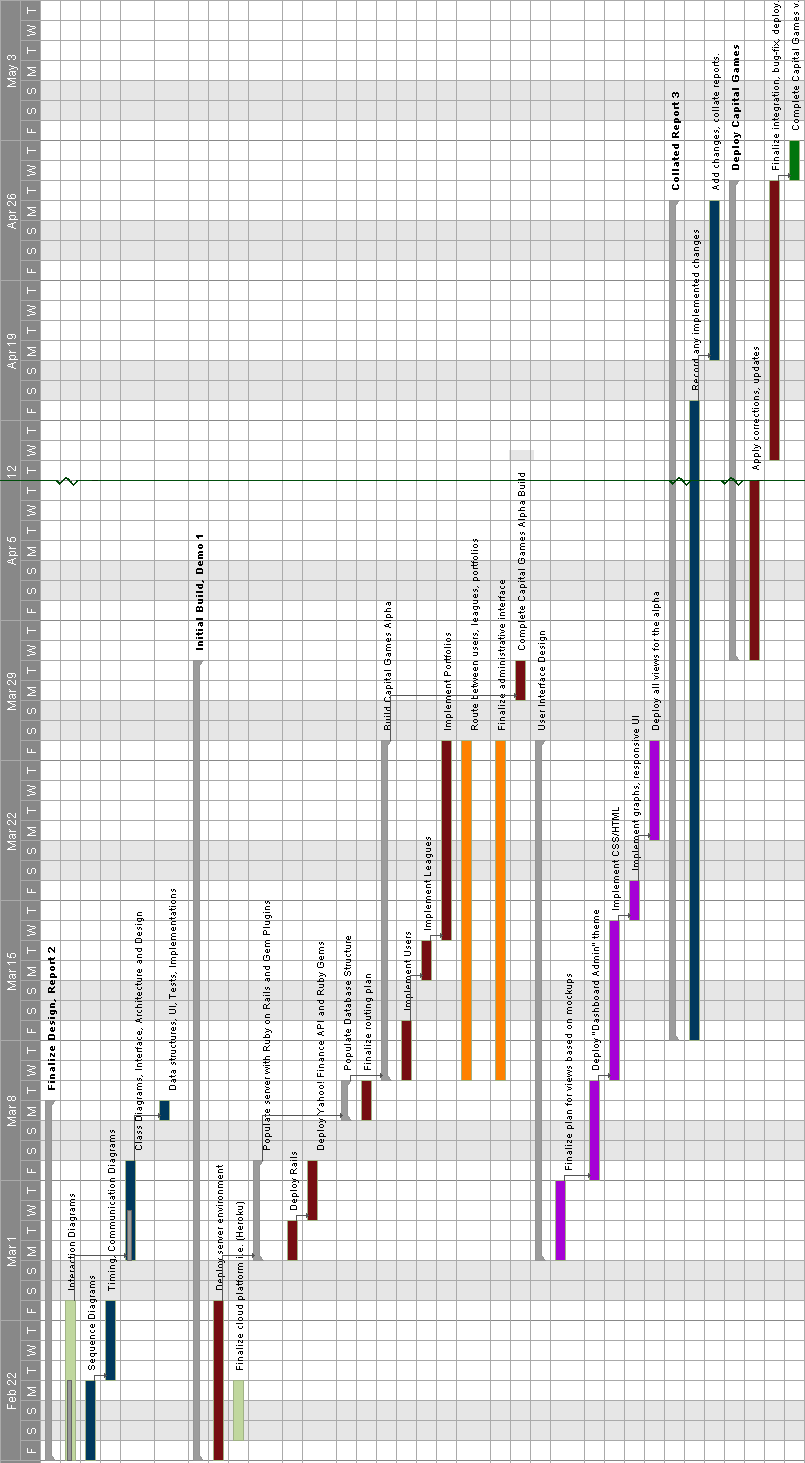
\includegraphics[width=7in]{./img/gantt.png}
\caption{This gantt chart projects how we will concurrently work on
the project. All blue items are report-related, red and orange relate
to the core project development and purple illustrates UI milestones.}
\end{figure}
% This chapter should include a Gantt chart for each our
% coding timelines for the first and second report and
% maybe even a second Gantt chart for our report deadlines
% from this report through May.
%
% Remember that we're trying to roll out core functionality 
% in time for the first demo, so try to include as much as 
% possible about creating users, leagues, basic settings (only),
% most trade and search things on the part for the first report,
% and the comments, reporting, adjusting settings, begin/end dates,
% privacy, mailing, whatever for the second. See our proposal for 
% the laundry list of features we actually said we'd be delivering.
%
% Also maybe talk about "Project Ownership", since he's big 
% on that. 
